\documentclass[12pt,letterspaper]{report}

\usepackage[spanish]{babel}
\usepackage[utf8]{inputenc}
\usepackage{graphicx}
\usepackage[T1]{fontenc}
\usepackage[latin1]{inputenc}
\usepackage[left=2.5cm, top=2.5cm, right=2.5cm, bottom=2.5cm]{geometry}



\title {Seguridad y Auditoria de Sistemas}
\author{ Ing. Melvin Kalí}


\begin{document}
\maketitle

\begin{titlepage}
\centering


\includegraphics[width=3cm, height=3cm]{Umg.jpg}


\vspace{1cm}
{\bfseries\LARGE Universidad Mariano Gálvez \par}
\vspace{1cm}
{\scshape\Large Facultad de Ingeniería En Sistemas \par}
\vspace{3cm}
{\scshape\Huge Proyecto Final \par}
\vspace{3cm}
{\itshape\Large Configuración de pfSense Firewall \par}
\vfill
{\Large Integrantes del Grupo: \par}
{\Large Rogelio Alfonso Alvarez Girón -- 7690-98-2290 \par}
{\Large Gari Lester Mendoza Bedoya -- 7690-17-14228 \par}
{\Large Selvin Omar Castellanos Solares 7690-17-14269} \par}
\vfill
{\Large Noviembre 2021 \par}
\end{titlepage}

\part {Configurando pfSense}
\chapter*{Configuraciónes realizadas}
A continuación veremos una serie de pasos que nos llevaron a configurar de una forma eficiente y segura el Firewall pfSense en nuestra red físico/virtual.

\section*{Instalación del Firewall}

Instalando pfSense Firewall: \par
\begin{itemize}

\item Hacemos boot en el equipo y en pocos segundos comienza la carga.

\item Aceptamos la licencia de uso y no distribución comercial presionando Enter

\item Llegamos al menú de bienvenida y contamos con 3 opciones
\end {itemize}

\begin {itemize}
\begin {enumerate}

\item Install: Comenzar los pasos de instalación (la que usaremos en este articulo)
\item Rescue Shell: Caer en el prompt del OS FreeBSD y realizar por comandos tareas de rescate o administración de nuestro cortafuegos
\item Recover config.xml: Restaurar un config.xml en un pfSense dañado o con problemas. Una forma útil de recuperarnos de un desastre
\end {enumerate}

Presionamos Enter sobre Install

\item Veremos un listado de distribuciones de teclado donde por medio del cursor bajaremos y buscaremos la que necesitemos.

\item En nuestro caso usaremos Latin American.

\item Presionamos Enter para marcarlo

\item De regreso al comienzo del listado podemos probar la distribución del teclado.

\item Usando la opción Test latinamerican.kbd keymap y despejar alguna duda de si es o no la que necesitamos.

\item Para continuar la instalación presionamos ENTER sobre --Continue with latinamerican.kbd keymap-- 
\end{itemize}


\part{Particionando disco de PfSense}
\chapter*{Descripción}
El asistente nos da 4 opciones para particionar el disco donde instalaremos

\begin{itemize}
\item Auto (UFS): La opción default, más sencilla, solo utilizara un disco
\item Manual: Particionaremos de forma manual, ideal para los casos en que compartiremos espacio con otra partición que no queremos eliminar
\item Shell: Realizar el particionado por línea de comandos en el shell
\item Auto (ZFS): Particionado con filesystem ZFS en 3 o mas discos, alta disponibilidad, mejor perfomance.
\end{itemize}

Bajamos con el cursor a Auto (ZFS) y presionamos Enter\par
\vspace {0.3cm}
La configuracion de ZFS puede parecer intimidante con tantas opciones pero no es de preocuparse, básicamente necesitamos solo decirle cuantos discos usaremos presionando Enter sobre T Pool Type/Disk
\vspace {0.3cm}
En la siguiente ventana veremos el listado de modos a elegir uno.

Algo muy útil, si tienes dudas de cual es el que puedes usar, con el cursor al pararte sobre una opción en la parte inferior te dice cuantos discos debes tener para su uso (Nota: los discos deben ser del mismo tamaño, de ponerle un disco mayor vas a malgastar el espacio extra).\par
\vspace {0.3cm}
Presionamos Enter \par
\vspace {0.3cm}
-Nos aparece el listado de discos, los marcamos con la tecla Espacio y presionamos Enter sobre OK para continuar\par

-De regreso a la ventana de configuracion de ZFS Configuration podríamos hacer otros cambios.\par
\vspace {0.3cm}
La recomendación, a no ser que lo necesiten, es que usen los valores default.\par
\vspace {0.3cm}
Presionamos Enter sobre Install\par
\vspace {0.3cm}
-Confirmamos el proceso presionando Enter sobre YES\par
\vspace {0.3cm}
-Comienza la instalación en disco.\par
\vspace {0.3cm}
-Si se quiere hacer algún otro cambio se puede hacer desde el shell por medio de comandos?\par
\vspace {0.3cm}
Presionamos Enter sobre No, para continuar\par
\vspace {0.3cm}
-Llegamos al final de la instalación.\par
\vspace {0.3cm}
Presionamos Enter sobre Reboot para reiniciar el equipo.\par
\vspace {0.3cm}
Quitamos el medio de instalación\par
\vspace {0.3cm}

\part{Configuración IP en pfSense}
\chapter*{Descripción}

-Apenas reiniciamos nuestro cortafuegos veremos la consola con opciones y las tarjetas de red auto configuradas.\par
\vspace {0.3cm}
Para este articulo en su modo básico (WAN y LAN) vemos que la WAN por default toma ip via DHCP (ideal para un esquema de cable modem o router de un ISP que asigne una ip).\par
\vspace {0.3cm}
La LAN se configura automáticamente con la 192.168.1.1.\par
\vspace {0.3cm}
Presionamos 2 y Enter\par
\vspace {0.3cm}
-Se nos da a elegir cual interfaz de red modificaremos, en este caso para cambiar la LAN elegimos 2 y presionamos Enter.\par
\vspace {0.3cm}
Seguidamente escribimos la IP que queremos activarle en la LAN.
\vspace {0.3cm}
Debes saber que esta sera la ip de puerta de salida o gateway a configurar en los equipos de tu LAN.\par
\vspace {0.3cm}
Dependiendo de tu esquema de red, elegimos la mascara, en mi caso usare 24 y presionamos Enter\par
\vspace {0.3cm}
-Como estamos modificando la IP LAN, en el siguiente paso no escribimos nada y presionamos Enter.\par
\vspace {0.3cm}
Si estuviéramos modificando WAN escribiríamos la ip del gateway o puerta de salida, generalmente una ip del router de nuestro proveedor internet.\par
\vspace {0.3cm}
Se nos pregunta si queremos revertir el protocolo para conectarnos via web, respondemos que n y presionamos Enter.\par
\vspace {0.3cm}
-El asistente nos confirma la activación de la nueva IP LAN y nos da el URL al que podemos acceder desde la LAN para su interfaz web.\par
\vspace {0.3cm}

\chapter*{Acceso al dashboard pfSense}
\vspace {0.1cm}
-Para acceder via web a nuestro cortafuegos abrimos un browser y navegamos a su URL https://IP-LAN-pfSense.\par
\vspace {0.3cm}
Recuerda que la ip por default LAN sera 192.168.1.1 pero si la modificaste la puedes confirmar en la consola texto.\par
\vspace {0.3cm}
Como el certificado SSL es auto firmado (es decir, no esta firmado por una entidad reconocida en internet dedicado a esto) tu navegador te puede dar un error .\par
\vspace {0.3cm}
No hay problema, damos click a Ocultar detalles avanzados y después a Continuar a 192.168.5.10 (no seguro).\par
\vspace {0.3cm}
En cualquier otro caso la IP seguramente será otra la ip\par
\vspace {0.3cm}
-Ingresamos por primera vez via web a pfSense, para eso usaremos los siguientes datos de usuario:\par
\vspace {0.3cm}
\begin{itemize}
\item usuario: \par
\item contraseña: \par
\end{itemize}
\vspace {0.3cm}
Y presionamos Enter o damos click al botón Sign in\par
\vspace {0.3cm}

\part{Setup pfSense}
\chapter*{Descripción}
\vspace {0.1cm}

-La primera vez que ingresemos via web a pfSense se ejecutara el Wizard pfSense Setup, usted elije si lo desea utilizar.\par
\vspace {0.3cm}
Este consta de 8 pasos desde el Inicio del wizard pfSense Setup.\par 
\vspace {0.3cm}

\begin{enumerate}
\item Ofrecimiento del soporte pago Netgate Global Support\par
\item Información general de nuestro cortafuegos\par
\item Activación de zona horaria para fecha y hora\par
\item Configuración interface WAN\par
\item Configuración interface LAN\par
\item Cambio de contraseña del usuario admin\par
\item Activar cambios.
\item Nuevamente se ofrece el soporte de Netgate finalizando el wizard\par
\end{enumerate}
\vspace {0.3cm}
Iniciamos el asistente.\par
\vspace {0.3cm}
Damos click al botón Next.\par
\vspace {0.3cm}
-En el primer paso se nos ofrece el soporte Netgate.\par
\vspace {0.3cm}
En caso de interesarte encentraras mas información dando click al botón Learn More.\par
\vspace {0.3cm}
Damos click al botón Next para continuar.\par
\vspace {0.3cm}
-Segundo paso, activamos el hostname y dominio de nuestro firewall ademas de los DNS primario y secundario.\par
\vspace {0.3cm}
Damos click al botón Next\par.
\vspace {0.3cm}
-Es importante que la fecha y hora de tu firewall estén sincronizados.\par
\vspace {0.3cm}
Eso lo hacemos en el tercer paso activando nuestra zona horaria en el campo Timezone.\par
\vspace {0.3cm}
Damos click al botón Next.\par
\vspace {0.3cm}
-Posiblemente el paso mas importante, el cuarto, donde configuraremos nuestra interfaz WAN.\par
\vspace {0.3cm}
Dependiendo de tu tipo de conexión sera la configuracion que harás.\par
\vspace {0.3cm}
Si usas DHCP para conectar tu pfSense Firewall a internet, entonces solo debes hacer ese cambio en el campo SelectType.\par
\vspace {0.3cm}
En caso de querer configurar otro tipo de conexión, se habilitaran otros campos a configurar.\par
\vspace {0.3cm}
Damos click al botón Next.\par
\vspace {0.3cm}
-Quinto paso, solo confirmar la IP LAN y su mascara.\par
\vspace {0.3cm}
Damos click al botón Next.\par
\vspace {0.3cm}
-No menos importante, en el sexto paso cambiamos la contraseña de la cuenta admin usada para conectarse al dashboard pfSense.\par
\vspace {0.3cm}
Damos click al botón Next.\par
\vspace {0.3cm}
-Realmente son 7 pasos, al llegar al séptimo paso ya habremos terminado, solo nos queda darle click al botón Reload para activar cambios.\par
\vspace {0.3cm}
-Es importante saber que no es permitido distribuir de forma comercial el software pfSense.\par
\vspace {0.3cm}
Aceptamos dando click al botón Accept.\par
\vspace {0.3cm}
-El dashboard web de pfSense Firewall es modular y en forma de bloques que nos irán dando información.\par
\vspace {0.3cm}

\part{Ilustraciones sobre la configuración}
\chapter*{Imagen 1}
\vspace {0.3cm}
\begin{figure}[htb]
\centering
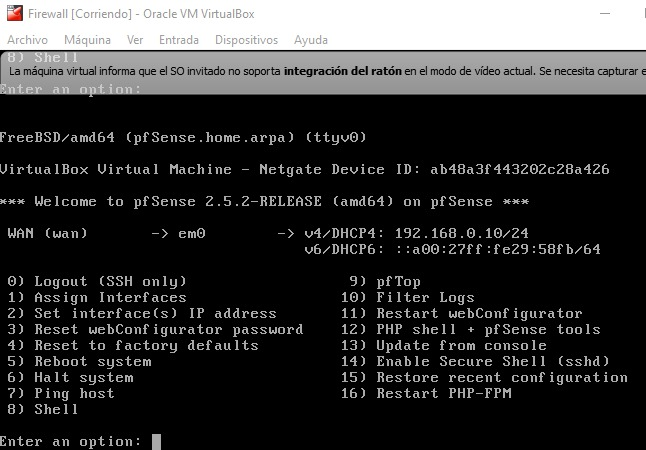
\includegraphics[scale=0.5]{Img1.jpg}
\caption{pfSenese corriendo en la máquina virtual}
\end{figure}\par
\vspace {0.1cm}


\chapter*{Imagen 2}
\vspace {0.3cm}
\begin{figure}[htb]
\centering
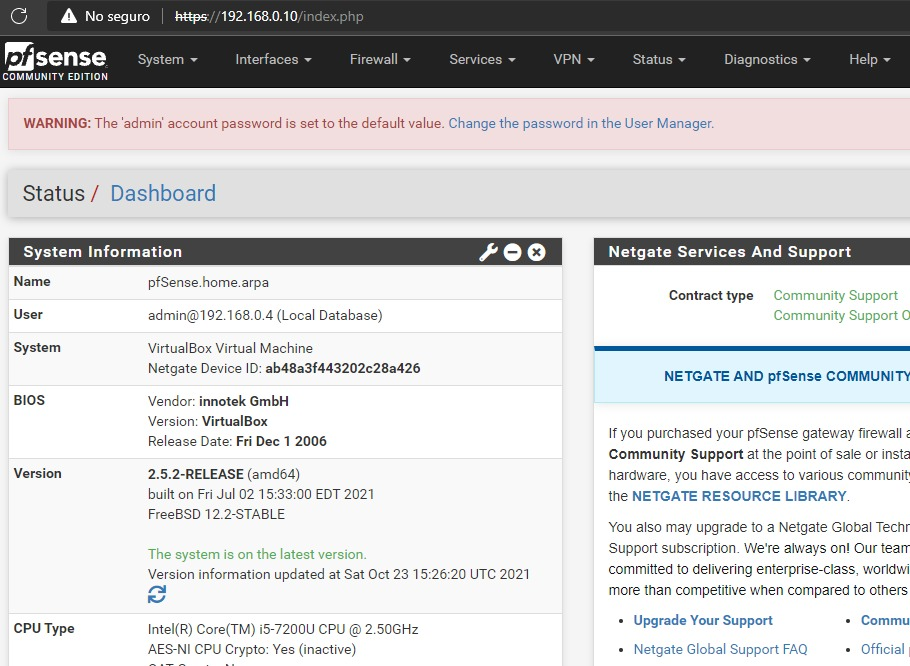
\includegraphics[scale=0.5]{Img2.jpg}
\caption{pfSenese en el navegador}
\end{figure}\par
\vspace {0.1cm}


\chapter*{Imagen 3}
\vspace {0.3cm}
\begin{figure}[htb]
\centering
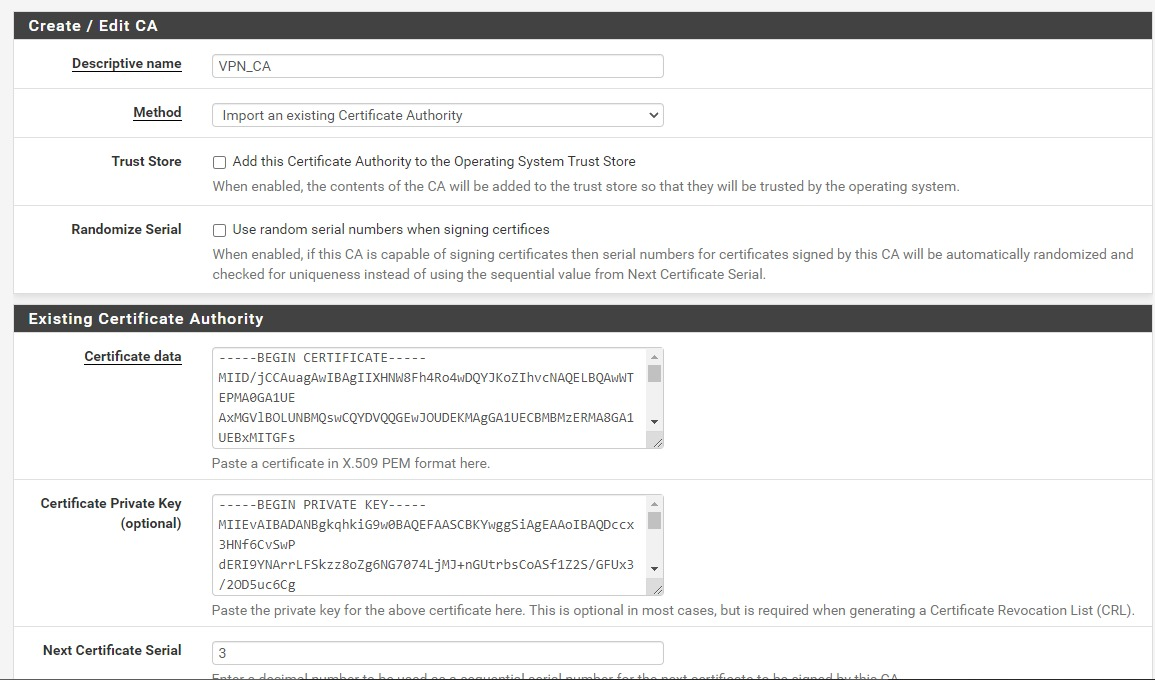
\includegraphics[scale=0.5]{Img3.jpg}
\caption{{Certificado del Servidor para crear nuevos certificados a usuarios}}
\end{figure}\par
\vspace {0.1cm}



\chapter*{Imagen 4}
\vspace {0.3cm}
\begin{figure}[htb]
\centering
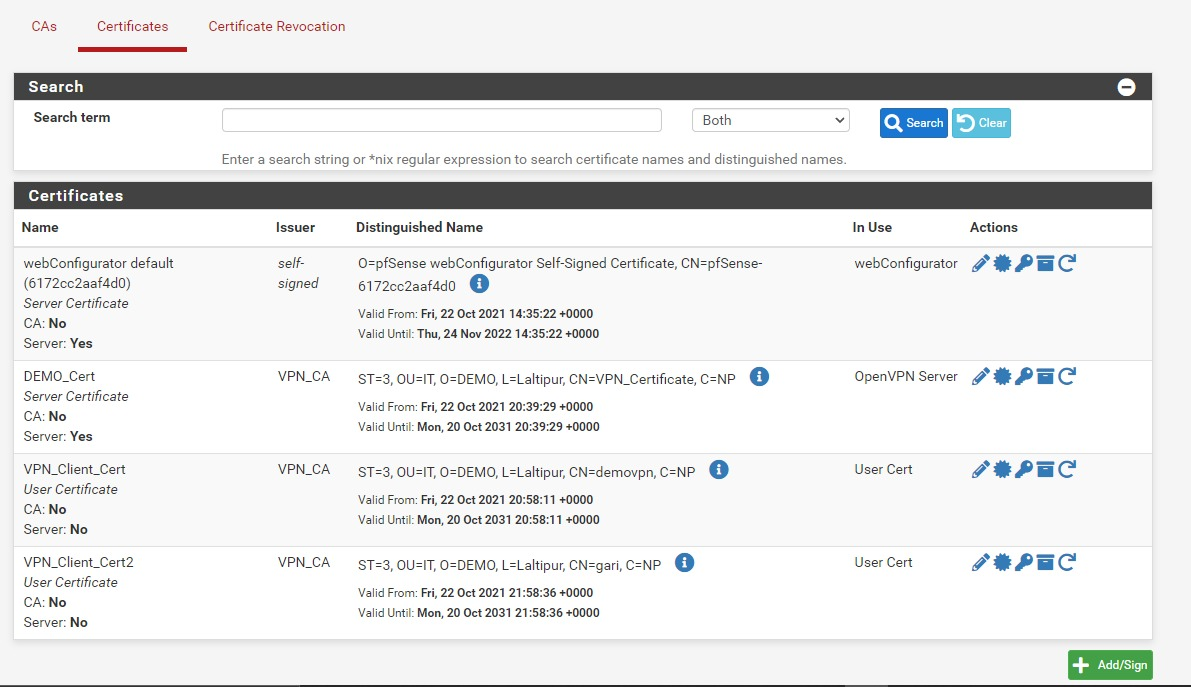
\includegraphics[scale=0.5]{Img4.jpg}
\caption{{Certificado existentes}}
\end{figure}\par
\vspace {0.1cm}



\chapter*{Imagen 5}
\vspace {0.3cm}
\begin{figure}[htb]
\centering
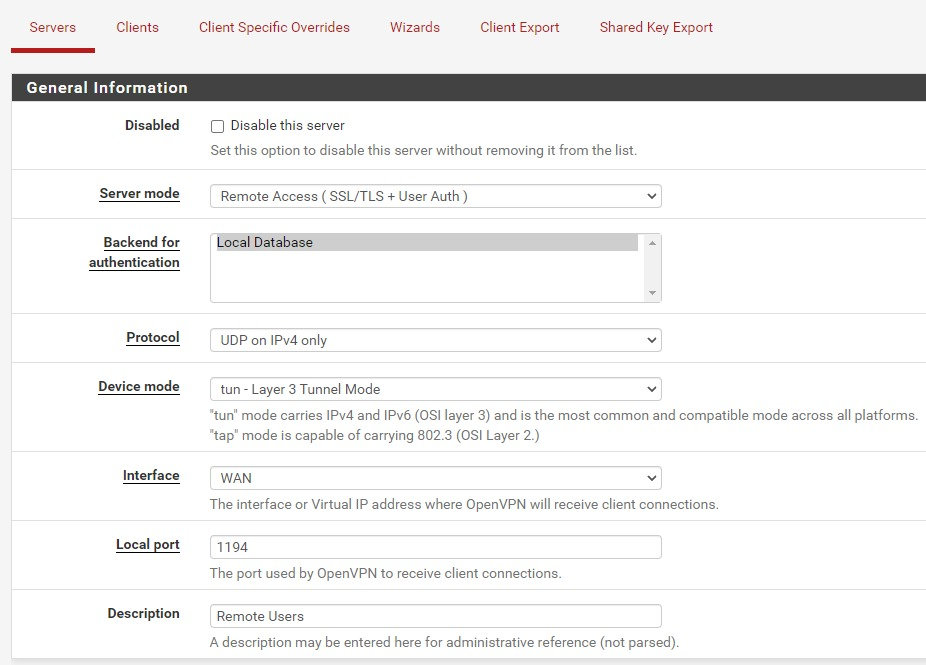
\includegraphics[scale=0.5]{Img5.jpg}
\caption{{Configuración del Servidor VPN en el Firewall}}
\end{figure}\par
\vspace {0.1cm}



\chapter*{Imagen 6}
\vspace {0.3cm}
\begin{figure}[htb]
\centering
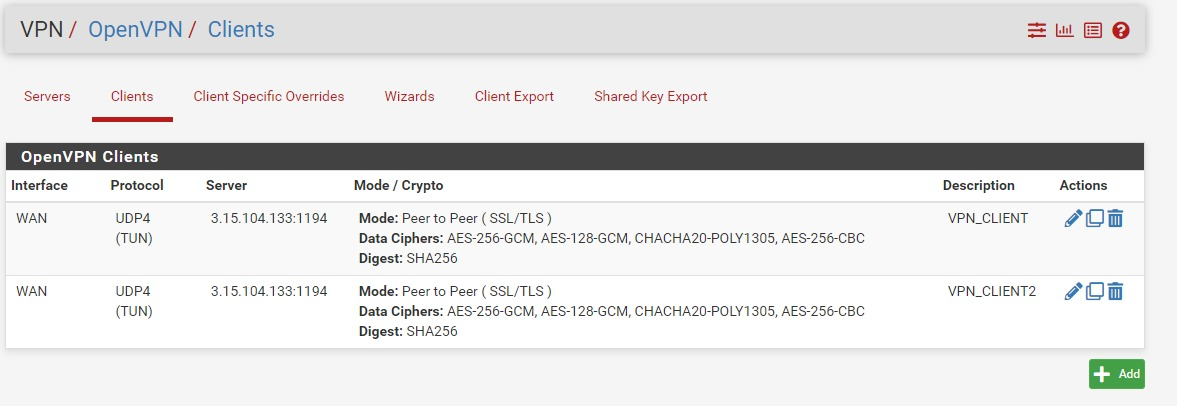
\includegraphics[scale=0.5]{Img6.jpg}
\caption{{Clientes creados en la VPN}}
\end{figure}\par
\vspace {0.1cm}


\chapter*{Imagen 7}
\vspace {0.3cm}
\begin{figure}[htb]
\centering
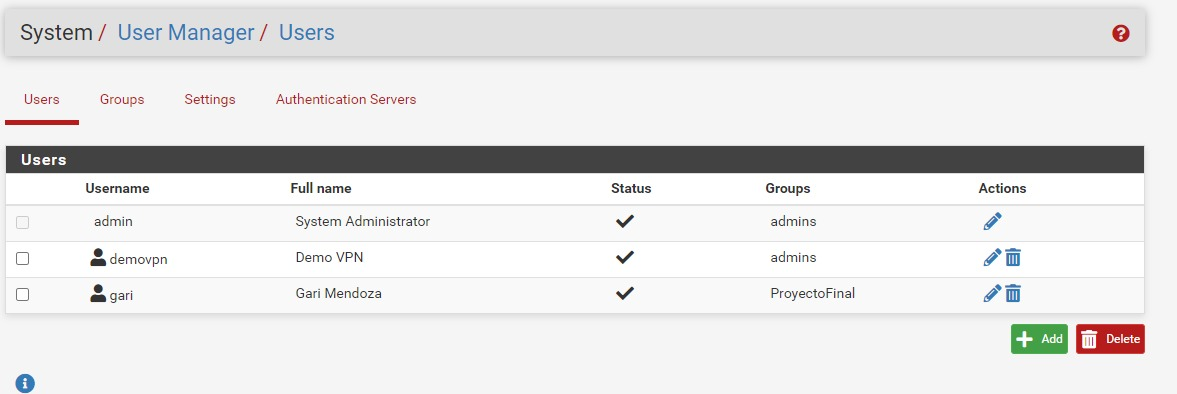
\includegraphics[scale=0.5]{Img7.jpg}
\caption{{Usuarios creados}}
\end{figure}\par
\vspace {0.1cm}

\chapter*{Imagen 8}
\vspace {0.3cm}
\begin{figure}[htb]
\centering
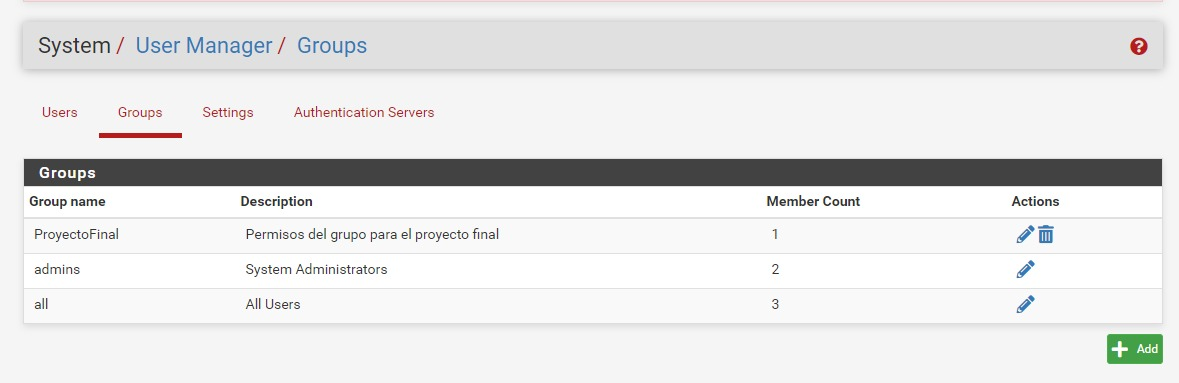
\includegraphics[scale=0.5]{Img8.jpg}
\caption{{Creación del grupo de Proyecto Final para el control de permisos limitados a usuarios}}
\end{figure}\par
\vspace {0.1cm}


\chapter*{Imagen 9}
\vspace {0.3cm}
\begin{figure}[htb]
\centering
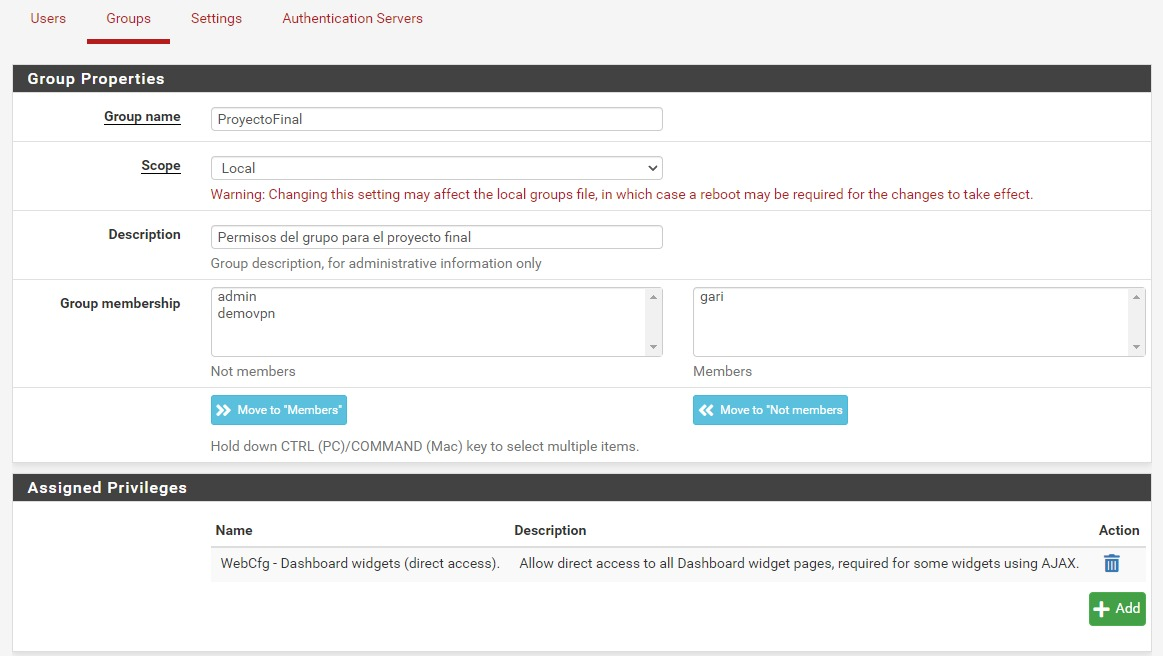
\includegraphics[scale=0.5]{Img9.jpg}
\caption{{Propiedades del grupo}}
\end{figure}\par
\vspace {0.1cm}


\chapter*{Imagen 10}
\vspace {0.3cm}
\begin{figure}[htb]
\centering
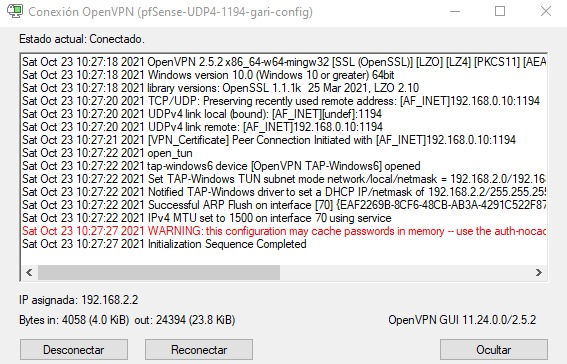
\includegraphics[scale=0.5]{Img10.jpg}
\caption{{Usuarios conectados con él usuario Gary y enlazados a la VPN}}
\end{figure}\par
\vspace {0.1cm}


\chapter*{Imagen 11}
\vspace {0.3cm}
\begin{figure}[htb]
\centering
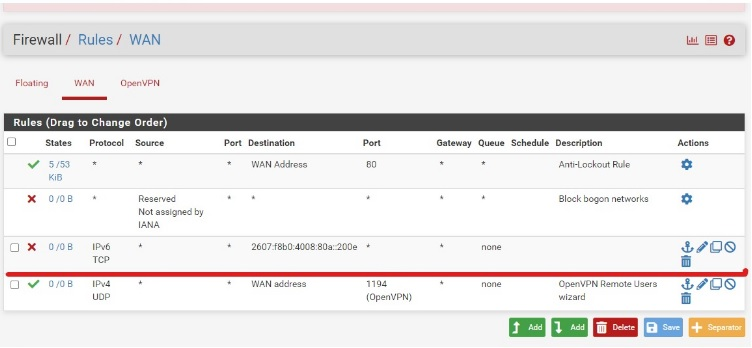
\includegraphics[scale=0.5]{Img11.jpg}
\caption{{Regla para bloquear Google}}
\end{figure}\par
\vspace {0.1cm}


\chapter*{Imagen 12}
\vspace {0.3cm}
\begin{figure}[htb]
\centering
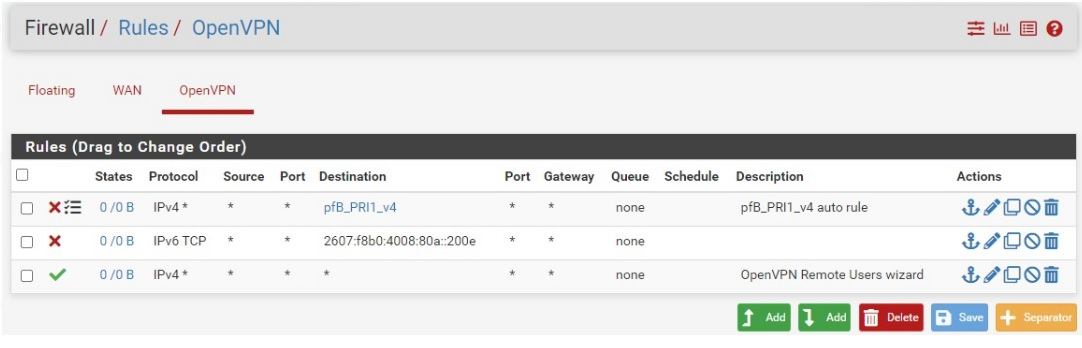
\includegraphics[scale=0.5]{Img12.jpg}
\caption{{Reglas para clientes que se conectan por la VPN}}
\end{figure}\par
\vspace {0.1cm}


\chapter*{Imagen 13}
\vspace {0.3cm}
\begin{figure}[htb]
\centering
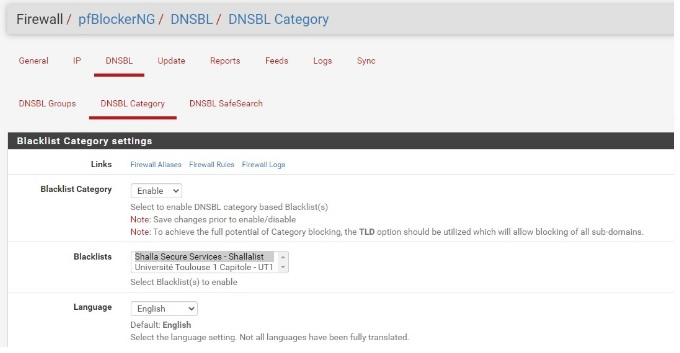
\includegraphics[scale=0.5]{Img13.jpg}
\caption{{pfBlockerNG elemento para bloquear paginas Web}}
\end{figure}\par
\vspace {0.1cm}


\chapter*{Imagen 14}
\vspace {0.3cm}
\begin{figure}[htb]
\centering
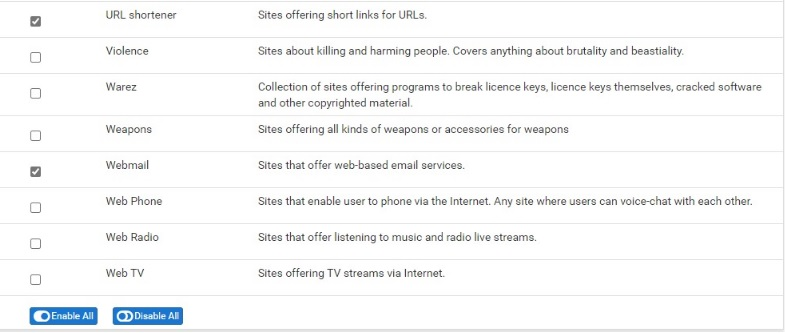
\includegraphics[scale=0.5]{Img14.jpg}
\caption{{Bloqueo de links que sean cortos}}
\end{figure}\par
\vspace {0.1cm}

\end{document}
